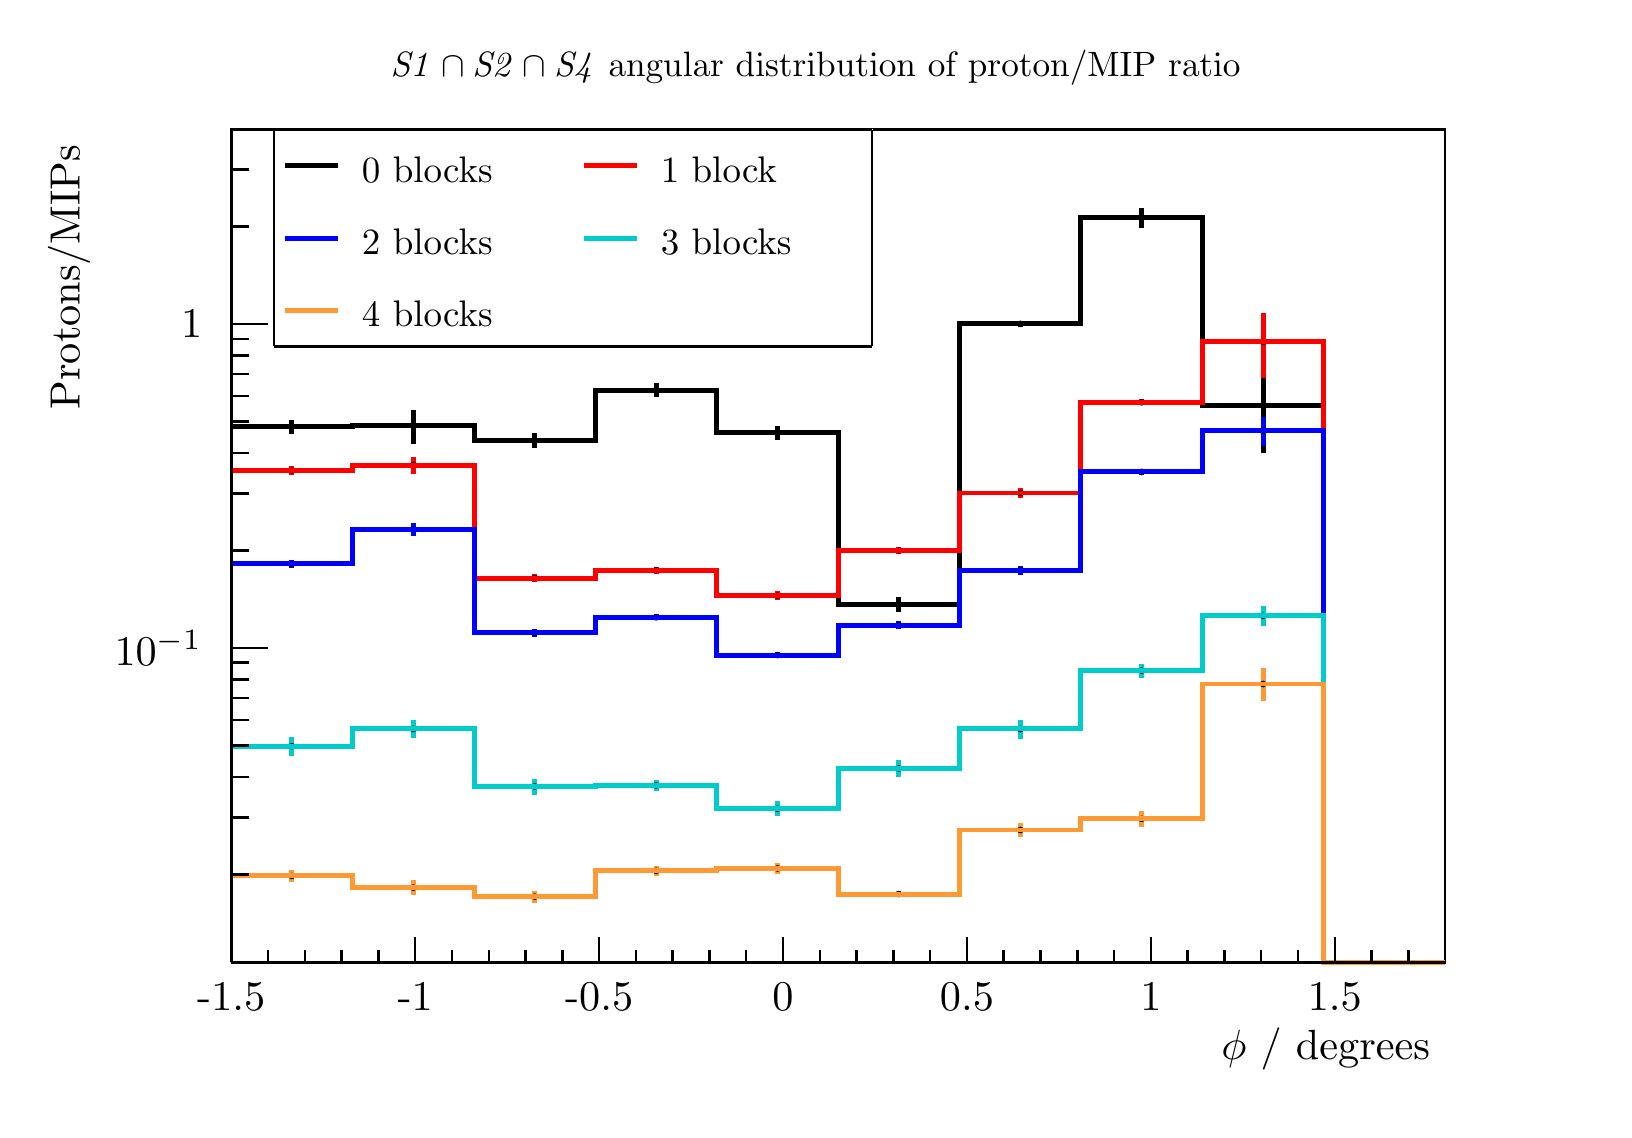
\begin{tikzpicture}
\pgfdeclareplotmark{cross} {
\pgfpathmoveto{\pgfpoint{-0.3\pgfplotmarksize}{\pgfplotmarksize}}
\pgfpathlineto{\pgfpoint{+0.3\pgfplotmarksize}{\pgfplotmarksize}}
\pgfpathlineto{\pgfpoint{+0.3\pgfplotmarksize}{0.3\pgfplotmarksize}}
\pgfpathlineto{\pgfpoint{+1\pgfplotmarksize}{0.3\pgfplotmarksize}}
\pgfpathlineto{\pgfpoint{+1\pgfplotmarksize}{-0.3\pgfplotmarksize}}
\pgfpathlineto{\pgfpoint{+0.3\pgfplotmarksize}{-0.3\pgfplotmarksize}}
\pgfpathlineto{\pgfpoint{+0.3\pgfplotmarksize}{-1.\pgfplotmarksize}}
\pgfpathlineto{\pgfpoint{-0.3\pgfplotmarksize}{-1.\pgfplotmarksize}}
\pgfpathlineto{\pgfpoint{-0.3\pgfplotmarksize}{-0.3\pgfplotmarksize}}
\pgfpathlineto{\pgfpoint{-1.\pgfplotmarksize}{-0.3\pgfplotmarksize}}
\pgfpathlineto{\pgfpoint{-1.\pgfplotmarksize}{0.3\pgfplotmarksize}}
\pgfpathlineto{\pgfpoint{-0.3\pgfplotmarksize}{0.3\pgfplotmarksize}}
\pgfpathclose
\pgfusepathqstroke
}
\pgfdeclareplotmark{cross*} {
\pgfpathmoveto{\pgfpoint{-0.3\pgfplotmarksize}{\pgfplotmarksize}}
\pgfpathlineto{\pgfpoint{+0.3\pgfplotmarksize}{\pgfplotmarksize}}
\pgfpathlineto{\pgfpoint{+0.3\pgfplotmarksize}{0.3\pgfplotmarksize}}
\pgfpathlineto{\pgfpoint{+1\pgfplotmarksize}{0.3\pgfplotmarksize}}
\pgfpathlineto{\pgfpoint{+1\pgfplotmarksize}{-0.3\pgfplotmarksize}}
\pgfpathlineto{\pgfpoint{+0.3\pgfplotmarksize}{-0.3\pgfplotmarksize}}
\pgfpathlineto{\pgfpoint{+0.3\pgfplotmarksize}{-1.\pgfplotmarksize}}
\pgfpathlineto{\pgfpoint{-0.3\pgfplotmarksize}{-1.\pgfplotmarksize}}
\pgfpathlineto{\pgfpoint{-0.3\pgfplotmarksize}{-0.3\pgfplotmarksize}}
\pgfpathlineto{\pgfpoint{-1.\pgfplotmarksize}{-0.3\pgfplotmarksize}}
\pgfpathlineto{\pgfpoint{-1.\pgfplotmarksize}{0.3\pgfplotmarksize}}
\pgfpathlineto{\pgfpoint{-0.3\pgfplotmarksize}{0.3\pgfplotmarksize}}
\pgfpathclose
\pgfusepathqfillstroke
}
\pgfdeclareplotmark{newstar} {
\pgfpathmoveto{\pgfqpoint{0pt}{\pgfplotmarksize}}
\pgfpathlineto{\pgfqpointpolar{44}{0.5\pgfplotmarksize}}
\pgfpathlineto{\pgfqpointpolar{18}{\pgfplotmarksize}}
\pgfpathlineto{\pgfqpointpolar{-20}{0.5\pgfplotmarksize}}
\pgfpathlineto{\pgfqpointpolar{-54}{\pgfplotmarksize}}
\pgfpathlineto{\pgfqpointpolar{-90}{0.5\pgfplotmarksize}}
\pgfpathlineto{\pgfqpointpolar{234}{\pgfplotmarksize}}
\pgfpathlineto{\pgfqpointpolar{198}{0.5\pgfplotmarksize}}
\pgfpathlineto{\pgfqpointpolar{162}{\pgfplotmarksize}}
\pgfpathlineto{\pgfqpointpolar{134}{0.5\pgfplotmarksize}}
\pgfpathclose
\pgfusepathqstroke
}
\pgfdeclareplotmark{newstar*} {
\pgfpathmoveto{\pgfqpoint{0pt}{\pgfplotmarksize}}
\pgfpathlineto{\pgfqpointpolar{44}{0.5\pgfplotmarksize}}
\pgfpathlineto{\pgfqpointpolar{18}{\pgfplotmarksize}}
\pgfpathlineto{\pgfqpointpolar{-20}{0.5\pgfplotmarksize}}
\pgfpathlineto{\pgfqpointpolar{-54}{\pgfplotmarksize}}
\pgfpathlineto{\pgfqpointpolar{-90}{0.5\pgfplotmarksize}}
\pgfpathlineto{\pgfqpointpolar{234}{\pgfplotmarksize}}
\pgfpathlineto{\pgfqpointpolar{198}{0.5\pgfplotmarksize}}
\pgfpathlineto{\pgfqpointpolar{162}{\pgfplotmarksize}}
\pgfpathlineto{\pgfqpointpolar{134}{0.5\pgfplotmarksize}}
\pgfpathclose
\pgfusepathqfillstroke
}
\definecolor{c}{rgb}{1,1,1};
\draw [color=c, fill=c] (0,0) rectangle (20,13.7249);
\draw [color=c, fill=c] (2.5788,1.86246) rectangle (17.9943,12.4355);
\definecolor{c}{rgb}{0,0,0};
\draw [c,line width=0.9] (2.5788,1.86246) -- (2.5788,12.4355) -- (17.9943,12.4355) -- (17.9943,1.86246) -- (2.5788,1.86246);
\definecolor{c}{rgb}{1,1,1};
\draw [color=c, fill=c] (2.5788,1.86246) rectangle (17.9943,12.4355);
\definecolor{c}{rgb}{0,0,0};
\draw [c,line width=0.9] (2.5788,1.86246) -- (2.5788,12.4355) -- (17.9943,12.4355) -- (17.9943,1.86246) -- (2.5788,1.86246);
\definecolor{c}{rgb}{0,0,0.6};
\draw [c,line width=0.9] (2.5788,1.86246) -- (4.12034,1.86246) -- (4.12034,1.86246) -- (5.66189,1.86246) -- (5.66189,1.86246) -- (7.20344,1.86246) -- (7.20344,1.86246) -- (8.74499,1.86246) -- (8.74499,1.86246) -- (10.2865,1.86246) --
 (10.2865,1.86246) -- (11.8281,1.86246) -- (11.8281,1.86246) -- (13.3696,1.86246) -- (13.3696,1.86246) -- (14.9112,1.86246) -- (14.9112,1.86246) -- (16.4527,1.86246) -- (16.4527,1.86246) -- (17.9943,1.86246);
\definecolor{c}{rgb}{0,0,0};
\draw [c,line width=0.9] (2.5788,1.86246) -- (17.9943,1.86246);
\draw [c,line width=0.9] (2.5788,2.17983) -- (2.5788,1.86246);
\draw [c,line width=0.9] (3.04593,2.02115) -- (3.04593,1.86246);
\draw [c,line width=0.9] (3.51307,2.02115) -- (3.51307,1.86246);
\draw [c,line width=0.9] (3.9802,2.02115) -- (3.9802,1.86246);
\draw [c,line width=0.9] (4.44734,2.02115) -- (4.44734,1.86246);
\draw [c,line width=0.9] (4.91447,2.17983) -- (4.91447,1.86246);
\draw [c,line width=0.9] (5.38161,2.02115) -- (5.38161,1.86246);
\draw [c,line width=0.9] (5.84875,2.02115) -- (5.84875,1.86246);
\draw [c,line width=0.9] (6.31588,2.02115) -- (6.31588,1.86246);
\draw [c,line width=0.9] (6.78302,2.02115) -- (6.78302,1.86246);
\draw [c,line width=0.9] (7.25015,2.17983) -- (7.25015,1.86246);
\draw [c,line width=0.9] (7.71729,2.02115) -- (7.71729,1.86246);
\draw [c,line width=0.9] (8.18442,2.02115) -- (8.18442,1.86246);
\draw [c,line width=0.9] (8.65156,2.02115) -- (8.65156,1.86246);
\draw [c,line width=0.9] (9.11869,2.02115) -- (9.11869,1.86246);
\draw [c,line width=0.9] (9.58583,2.17983) -- (9.58583,1.86246);
\draw [c,line width=0.9] (10.053,2.02115) -- (10.053,1.86246);
\draw [c,line width=0.9] (10.5201,2.02115) -- (10.5201,1.86246);
\draw [c,line width=0.9] (10.9872,2.02115) -- (10.9872,1.86246);
\draw [c,line width=0.9] (11.4544,2.02115) -- (11.4544,1.86246);
\draw [c,line width=0.9] (11.9215,2.17983) -- (11.9215,1.86246);
\draw [c,line width=0.9] (12.3886,2.02115) -- (12.3886,1.86246);
\draw [c,line width=0.9] (12.8558,2.02115) -- (12.8558,1.86246);
\draw [c,line width=0.9] (13.3229,2.02115) -- (13.3229,1.86246);
\draw [c,line width=0.9] (13.79,2.02115) -- (13.79,1.86246);
\draw [c,line width=0.9] (14.2572,2.17983) -- (14.2572,1.86246);
\draw [c,line width=0.9] (14.7243,2.02115) -- (14.7243,1.86246);
\draw [c,line width=0.9] (15.1915,2.02115) -- (15.1915,1.86246);
\draw [c,line width=0.9] (15.6586,2.02115) -- (15.6586,1.86246);
\draw [c,line width=0.9] (16.1257,2.02115) -- (16.1257,1.86246);
\draw [c,line width=0.9] (16.5929,2.17983) -- (16.5929,1.86246);
\draw [c,line width=0.9] (16.5929,2.17983) -- (16.5929,1.86246);
\draw [c,line width=0.9] (17.06,2.02115) -- (17.06,1.86246);
\draw [c,line width=0.9] (17.5271,2.02115) -- (17.5271,1.86246);
\draw [anchor=base] (2.5788,1.24484) node[scale=1.52731, color=c, rotate=0]{-1.5};
\draw [anchor=base] (4.91447,1.24484) node[scale=1.52731, color=c, rotate=0]{-1};
\draw [anchor=base] (7.25015,1.24484) node[scale=1.52731, color=c, rotate=0]{-0.5};
\draw [anchor=base] (9.58583,1.24484) node[scale=1.52731, color=c, rotate=0]{0};
\draw [anchor=base] (11.9215,1.24484) node[scale=1.52731, color=c, rotate=0]{0.5};
\draw [anchor=base] (14.2572,1.24484) node[scale=1.52731, color=c, rotate=0]{1};
\draw [anchor=base] (16.5929,1.24484) node[scale=1.52731, color=c, rotate=0]{1.5};
\draw [anchor= east] (17.9943,0.76447) node[scale=1.52731, color=c, rotate=0]{$ \phi$ / degrees};
\draw [c,line width=0.9] (2.5788,1.86246) -- (2.5788,12.4355);
\draw [c,line width=0.9] (2.8099,2.97941) -- (2.5788,2.97941);
\draw [c,line width=0.9] (2.8099,3.70388) -- (2.5788,3.70388);
\draw [c,line width=0.9] (2.8099,4.2179) -- (2.5788,4.2179);
\draw [c,line width=0.9] (2.8099,4.61661) -- (2.5788,4.61661);
\draw [c,line width=0.9] (2.8099,4.94238) -- (2.5788,4.94238);
\draw [c,line width=0.9] (2.8099,5.21781) -- (2.5788,5.21781);
\draw [c,line width=0.9] (2.8099,5.4564) -- (2.5788,5.4564);
\draw [c,line width=0.9] (2.8099,5.66685) -- (2.5788,5.66685);
\draw [c,line width=0.9] (3.04101,5.8551) -- (2.5788,5.8551);
\draw [anchor= east] (2.3988,5.8551) node[scale=1.52731, color=c, rotate=0]{$10^{-1}$};
\draw [c,line width=0.9] (2.8099,7.0936) -- (2.5788,7.0936);
\draw [c,line width=0.9] (2.8099,7.81807) -- (2.5788,7.81807);
\draw [c,line width=0.9] (2.8099,8.3321) -- (2.5788,8.3321);
\draw [c,line width=0.9] (2.8099,8.7308) -- (2.5788,8.7308);
\draw [c,line width=0.9] (2.8099,9.05657) -- (2.5788,9.05657);
\draw [c,line width=0.9] (2.8099,9.332) -- (2.5788,9.332);
\draw [c,line width=0.9] (2.8099,9.57059) -- (2.5788,9.57059);
\draw [c,line width=0.9] (2.8099,9.78104) -- (2.5788,9.78104);
\draw [c,line width=0.9] (3.04101,9.9693) -- (2.5788,9.9693);
\draw [anchor= east] (2.3988,9.9693) node[scale=1.52731, color=c, rotate=0]{1};
\draw [c,line width=0.9] (2.8099,11.2078) -- (2.5788,11.2078);
\draw [c,line width=0.9] (2.8099,11.9323) -- (2.5788,11.9323);
\draw [anchor= east] (0.518624,12.4355) node[scale=1.52731, color=c, rotate=90]{ Protons/MIPs};
\draw [c,line width=1.8] (3.34957,8.57001) -- (3.34957,8.66425);
\draw [c,line width=1.8] (3.34957,8.66425) -- (3.34957,8.75377);
\foreach \P in {(3.34957,8.66425)}{\draw[mark options={color=c,fill=c},mark size=2.402402pt,mark=*,mark size=1pt] plot coordinates {\P};}
\draw [c,line width=1.8] (4.89112,8.44714) -- (4.89112,8.6769);
\draw [c,line width=1.8] (4.89112,8.6769) -- (4.89112,8.88046);
\foreach \P in {(4.89112,8.6769)}{\draw[mark options={color=c,fill=c},mark size=2.402402pt,mark=*,mark size=1pt] plot coordinates {\P};}
\draw [c,line width=1.8] (6.43266,8.39359) -- (6.43266,8.49235);
\draw [c,line width=1.8] (6.43266,8.49235) -- (6.43266,8.58594);
\foreach \P in {(6.43266,8.49235)}{\draw[mark options={color=c,fill=c},mark size=2.402402pt,mark=*,mark size=1pt] plot coordinates {\P};}
\draw [c,line width=1.8] (7.97421,9.03898) -- (7.97421,9.12998);
\draw [c,line width=1.8] (7.97421,9.12998) -- (7.97421,9.21658);
\foreach \P in {(7.97421,9.12998)}{\draw[mark options={color=c,fill=c},mark size=2.402402pt,mark=*,mark size=1pt] plot coordinates {\P};}
\draw [c,line width=1.8] (9.51576,8.49573) -- (9.51576,8.5843);
\draw [c,line width=1.8] (9.51576,8.5843) -- (9.51576,8.66868);
\foreach \P in {(9.51576,8.5843)}{\draw[mark options={color=c,fill=c},mark size=2.402402pt,mark=*,mark size=1pt] plot coordinates {\P};}
\draw [c,line width=1.8] (11.0573,6.31434) -- (11.0573,6.40994);
\draw [c,line width=1.8] (11.0573,6.40994) -- (11.0573,6.50069);
\foreach \P in {(11.0573,6.40994)}{\draw[mark options={color=c,fill=c},mark size=2.402402pt,mark=*,mark size=1pt] plot coordinates {\P};}
\draw [c,line width=1.8] (12.5989,9.92745) -- (12.5989,9.97028);
\draw [c,line width=1.8] (12.5989,9.97028) -- (12.5989,10.0121);
\foreach \P in {(12.5989,9.97028)}{\draw[mark options={color=c,fill=c},mark size=2.402402pt,mark=*,mark size=1pt] plot coordinates {\P};}
\draw [c,line width=1.8] (14.1404,11.189) -- (14.1404,11.3184);
\draw [c,line width=1.8] (14.1404,11.3184) -- (14.1404,11.4391);
\foreach \P in {(14.1404,11.3184)}{\draw[mark options={color=c,fill=c},mark size=2.402402pt,mark=*,mark size=1pt] plot coordinates {\P};}
\draw [c,line width=1.8] (15.6819,8.32773) -- (15.6819,8.92976);
\draw [c,line width=1.8] (15.6819,8.92976) -- (15.6819,9.37926);
\foreach \P in {(15.6819,8.92976)}{\draw[mark options={color=c,fill=c},mark size=2.402402pt,mark=*,mark size=1pt] plot coordinates {\P};}
\draw [c,line width=1.8] (2.5788,8.66425) -- (4.12034,8.66425) -- (4.12034,8.6769) -- (5.66189,8.6769) -- (5.66189,8.49235) -- (7.20344,8.49235) -- (7.20344,9.12998) -- (8.74499,9.12998) -- (8.74499,8.5843) -- (10.2865,8.5843) -- (10.2865,6.40994) --
 (11.8281,6.40994) -- (11.8281,9.97028) -- (13.3696,9.97028) -- (13.3696,11.3184) -- (14.9112,11.3184) -- (14.9112,8.92976) -- (16.4527,8.92976) -- (16.4527,1.86246) -- (17.9943,1.86246);
\definecolor{c}{rgb}{1,0,0};
\draw [c,line width=1.8] (3.34957,8.05322) -- (3.34957,8.10767);
\draw [c,line width=1.8] (3.34957,8.10767) -- (3.34957,8.1605);
\definecolor{c}{rgb}{0,0,0};
\foreach \P in {(3.34957,8.10767)}{\draw[mark options={color=c,fill=c},mark size=2.402402pt,mark=*,mark size=1pt] plot coordinates {\P};}
\definecolor{c}{rgb}{1,0,0};
\draw [c,line width=1.8] (4.89112,8.06202) -- (4.89112,8.17703);
\draw [c,line width=1.8] (4.89112,8.17703) -- (4.89112,8.28509);
\definecolor{c}{rgb}{0,0,0};
\foreach \P in {(4.89112,8.17703)}{\draw[mark options={color=c,fill=c},mark size=2.402402pt,mark=*,mark size=1pt] plot coordinates {\P};}
\definecolor{c}{rgb}{1,0,0};
\draw [c,line width=1.8] (6.43266,6.69263) -- (6.43266,6.74056);
\draw [c,line width=1.8] (6.43266,6.74056) -- (6.43266,6.78723);
\definecolor{c}{rgb}{0,0,0};
\foreach \P in {(6.43266,6.74056)}{\draw[mark options={color=c,fill=c},mark size=2.402402pt,mark=*,mark size=1pt] plot coordinates {\P};}
\definecolor{c}{rgb}{1,0,0};
\draw [c,line width=1.8] (7.97421,6.79689) -- (7.97421,6.84261);
\draw [c,line width=1.8] (7.97421,6.84261) -- (7.97421,6.88718);
\definecolor{c}{rgb}{0,0,0};
\foreach \P in {(7.97421,6.84261)}{\draw[mark options={color=c,fill=c},mark size=2.402402pt,mark=*,mark size=1pt] plot coordinates {\P};}
\definecolor{c}{rgb}{1,0,0};
\draw [c,line width=1.8] (9.51576,6.46031) -- (9.51576,6.518);
\draw [c,line width=1.8] (9.51576,6.518) -- (9.51576,6.57388);
\definecolor{c}{rgb}{0,0,0};
\foreach \P in {(9.51576,6.518)}{\draw[mark options={color=c,fill=c},mark size=2.402402pt,mark=*,mark size=1pt] plot coordinates {\P};}
\definecolor{c}{rgb}{1,0,0};
\draw [c,line width=1.8] (11.0573,7.0412) -- (11.0573,7.09145);
\draw [c,line width=1.8] (11.0573,7.09145) -- (11.0573,7.14034);
\definecolor{c}{rgb}{0,0,0};
\foreach \P in {(11.0573,7.09145)}{\draw[mark options={color=c,fill=c},mark size=2.402402pt,mark=*,mark size=1pt] plot coordinates {\P};}
\definecolor{c}{rgb}{1,0,0};
\draw [c,line width=1.8] (12.5989,7.76328) -- (12.5989,7.82227);
\draw [c,line width=1.8] (12.5989,7.82227) -- (12.5989,7.87937);
\definecolor{c}{rgb}{0,0,0};
\foreach \P in {(12.5989,7.82227)}{\draw[mark options={color=c,fill=c},mark size=2.402402pt,mark=*,mark size=1pt] plot coordinates {\P};}
\definecolor{c}{rgb}{1,0,0};
\draw [c,line width=1.8] (14.1404,8.93398) -- (14.1404,8.97442);
\draw [c,line width=1.8] (14.1404,8.97442) -- (14.1404,9.01396);
\definecolor{c}{rgb}{0,0,0};
\foreach \P in {(14.1404,8.97442)}{\draw[mark options={color=c,fill=c},mark size=2.402402pt,mark=*,mark size=1pt] plot coordinates {\P};}
\definecolor{c}{rgb}{1,0,0};
\draw [c,line width=1.8] (15.6819,9.28528) -- (15.6819,9.74231);
\draw [c,line width=1.8] (15.6819,9.74231) -- (15.6819,10.1059);
\definecolor{c}{rgb}{0,0,0};
\foreach \P in {(15.6819,9.74231)}{\draw[mark options={color=c,fill=c},mark size=2.402402pt,mark=*,mark size=1pt] plot coordinates {\P};}
\definecolor{c}{rgb}{1,0,0};
\draw [c,line width=1.8] (2.5788,8.10767) -- (4.12034,8.10767) -- (4.12034,8.17703) -- (5.66189,8.17703) -- (5.66189,6.74056) -- (7.20344,6.74056) -- (7.20344,6.84261) -- (8.74499,6.84261) -- (8.74499,6.518) -- (10.2865,6.518) -- (10.2865,7.09145) --
 (11.8281,7.09145) -- (11.8281,7.82227) -- (13.3696,7.82227) -- (13.3696,8.97442) -- (14.9112,8.97442) -- (14.9112,9.74231) -- (16.4527,9.74231) -- (16.4527,1.86246) -- (17.9943,1.86246);
\definecolor{c}{rgb}{0,0,1};
\draw [c,line width=1.8] (3.34957,6.86652) -- (3.34957,6.92165);
\draw [c,line width=1.8] (3.34957,6.92165) -- (3.34957,6.97514);
\definecolor{c}{rgb}{0,0,0};
\foreach \P in {(3.34957,6.92165)}{\draw[mark options={color=c,fill=c},mark size=2.402402pt,mark=*,mark size=1pt] plot coordinates {\P};}
\definecolor{c}{rgb}{0,0,1};
\draw [c,line width=1.8] (4.89112,7.27615) -- (4.89112,7.36159);
\draw [c,line width=1.8] (4.89112,7.36159) -- (4.89112,7.44313);
\definecolor{c}{rgb}{0,0,0};
\foreach \P in {(4.89112,7.36159)}{\draw[mark options={color=c,fill=c},mark size=2.402402pt,mark=*,mark size=1pt] plot coordinates {\P};}
\definecolor{c}{rgb}{0,0,1};
\draw [c,line width=1.8] (6.43266,5.99417) -- (6.43266,6.04779);
\draw [c,line width=1.8] (6.43266,6.04779) -- (6.43266,6.09984);
\definecolor{c}{rgb}{0,0,0};
\foreach \P in {(6.43266,6.04779)}{\draw[mark options={color=c,fill=c},mark size=2.402402pt,mark=*,mark size=1pt] plot coordinates {\P};}
\definecolor{c}{rgb}{0,0,1};
\draw [c,line width=1.8] (7.97421,6.20509) -- (7.97421,6.24398);
\draw [c,line width=1.8] (7.97421,6.24398) -- (7.97421,6.28204);
\definecolor{c}{rgb}{0,0,0};
\foreach \P in {(7.97421,6.24398)}{\draw[mark options={color=c,fill=c},mark size=2.402402pt,mark=*,mark size=1pt] plot coordinates {\P};}
\definecolor{c}{rgb}{0,0,1};
\draw [c,line width=1.8] (9.51576,5.72213) -- (9.51576,5.76439);
\draw [c,line width=1.8] (9.51576,5.76439) -- (9.51576,5.80568);
\definecolor{c}{rgb}{0,0,0};
\foreach \P in {(9.51576,5.76439)}{\draw[mark options={color=c,fill=c},mark size=2.402402pt,mark=*,mark size=1pt] plot coordinates {\P};}
\definecolor{c}{rgb}{0,0,1};
\draw [c,line width=1.8] (11.0573,6.0978) -- (11.0573,6.14558);
\draw [c,line width=1.8] (11.0573,6.14558) -- (11.0573,6.1921);
\definecolor{c}{rgb}{0,0,0};
\foreach \P in {(11.0573,6.14558)}{\draw[mark options={color=c,fill=c},mark size=2.402402pt,mark=*,mark size=1pt] plot coordinates {\P};}
\definecolor{c}{rgb}{0,0,1};
\draw [c,line width=1.8] (12.5989,6.78221) -- (12.5989,6.84262);
\draw [c,line width=1.8] (12.5989,6.84262) -- (12.5989,6.90105);
\definecolor{c}{rgb}{0,0,0};
\foreach \P in {(12.5989,6.84262)}{\draw[mark options={color=c,fill=c},mark size=2.402402pt,mark=*,mark size=1pt] plot coordinates {\P};}
\definecolor{c}{rgb}{0,0,1};
\draw [c,line width=1.8] (14.1404,8.04737) -- (14.1404,8.09002);
\draw [c,line width=1.8] (14.1404,8.09002) -- (14.1404,8.13167);
\definecolor{c}{rgb}{0,0,0};
\foreach \P in {(14.1404,8.09002)}{\draw[mark options={color=c,fill=c},mark size=2.402402pt,mark=*,mark size=1pt] plot coordinates {\P};}
\definecolor{c}{rgb}{0,0,1};
\draw [c,line width=1.8] (15.6819,8.4153) -- (15.6819,8.61154);
\draw [c,line width=1.8] (15.6819,8.61154) -- (15.6819,8.78835);
\definecolor{c}{rgb}{0,0,0};
\foreach \P in {(15.6819,8.61154)}{\draw[mark options={color=c,fill=c},mark size=2.402402pt,mark=*,mark size=1pt] plot coordinates {\P};}
\definecolor{c}{rgb}{0,0,1};
\draw [c,line width=1.8] (2.5788,6.92165) -- (4.12034,6.92165) -- (4.12034,7.36159) -- (5.66189,7.36159) -- (5.66189,6.04779) -- (7.20344,6.04779) -- (7.20344,6.24398) -- (8.74499,6.24398) -- (8.74499,5.76439) -- (10.2865,5.76439) --
 (10.2865,6.14558) -- (11.8281,6.14558) -- (11.8281,6.84262) -- (13.3696,6.84262) -- (13.3696,8.09002) -- (14.9112,8.09002) -- (14.9112,8.61154) -- (16.4527,8.61154) -- (16.4527,1.86246) -- (17.9943,1.86246);
\definecolor{c}{rgb}{0,0.8,0.8};
\draw [c,line width=1.8] (3.34957,4.4818) -- (3.34957,4.60711);
\draw [c,line width=1.8] (3.34957,4.60711) -- (3.34957,4.72421);
\definecolor{c}{rgb}{0,0,0};
\foreach \P in {(3.34957,4.60711)}{\draw[mark options={color=c,fill=c},mark size=2.402402pt,mark=*,mark size=1pt] plot coordinates {\P};}
\definecolor{c}{rgb}{0,0.8,0.8};
\draw [c,line width=1.8] (4.89112,4.71153) -- (4.89112,4.82697);
\draw [c,line width=1.8] (4.89112,4.82697) -- (4.89112,4.9354);
\definecolor{c}{rgb}{0,0,0};
\foreach \P in {(4.89112,4.82697)}{\draw[mark options={color=c,fill=c},mark size=2.402402pt,mark=*,mark size=1pt] plot coordinates {\P};}
\definecolor{c}{rgb}{0,0.8,0.8};
\draw [c,line width=1.8] (6.43266,3.98915) -- (6.43266,4.09539);
\draw [c,line width=1.8] (6.43266,4.09539) -- (6.43266,4.19566);
\definecolor{c}{rgb}{0,0,0};
\foreach \P in {(6.43266,4.09539)}{\draw[mark options={color=c,fill=c},mark size=2.402402pt,mark=*,mark size=1pt] plot coordinates {\P};}
\definecolor{c}{rgb}{0,0.8,0.8};
\draw [c,line width=1.8] (7.97421,4.03233) -- (7.97421,4.10899);
\draw [c,line width=1.8] (7.97421,4.10899) -- (7.97421,4.18251);
\definecolor{c}{rgb}{0,0,0};
\foreach \P in {(7.97421,4.10899)}{\draw[mark options={color=c,fill=c},mark size=2.402402pt,mark=*,mark size=1pt] plot coordinates {\P};}
\definecolor{c}{rgb}{0,0.8,0.8};
\draw [c,line width=1.8] (9.51576,3.71388) -- (9.51576,3.81207);
\draw [c,line width=1.8] (9.51576,3.81207) -- (9.51576,3.90515);
\definecolor{c}{rgb}{0,0,0};
\foreach \P in {(9.51576,3.81207)}{\draw[mark options={color=c,fill=c},mark size=2.402402pt,mark=*,mark size=1pt] plot coordinates {\P};}
\definecolor{c}{rgb}{0,0.8,0.8};
\draw [c,line width=1.8] (11.0573,4.21161) -- (11.0573,4.32441);
\draw [c,line width=1.8] (11.0573,4.32441) -- (11.0573,4.43051);
\definecolor{c}{rgb}{0,0,0};
\foreach \P in {(11.0573,4.32441)}{\draw[mark options={color=c,fill=c},mark size=2.402402pt,mark=*,mark size=1pt] plot coordinates {\P};}
\definecolor{c}{rgb}{0,0.8,0.8};
\draw [c,line width=1.8] (12.5989,4.70291) -- (12.5989,4.82515);
\draw [c,line width=1.8] (12.5989,4.82515) -- (12.5989,4.93956);
\definecolor{c}{rgb}{0,0,0};
\foreach \P in {(12.5989,4.82515)}{\draw[mark options={color=c,fill=c},mark size=2.402402pt,mark=*,mark size=1pt] plot coordinates {\P};}
\definecolor{c}{rgb}{0,0.8,0.8};
\draw [c,line width=1.8] (14.1404,5.47244) -- (14.1404,5.56633);
\draw [c,line width=1.8] (14.1404,5.56633) -- (14.1404,5.65553);
\definecolor{c}{rgb}{0,0,0};
\foreach \P in {(14.1404,5.56633)}{\draw[mark options={color=c,fill=c},mark size=2.402402pt,mark=*,mark size=1pt] plot coordinates {\P};}
\definecolor{c}{rgb}{0,0.8,0.8};
\draw [c,line width=1.8] (15.6819,6.13114) -- (15.6819,6.26276);
\draw [c,line width=1.8] (15.6819,6.26276) -- (15.6819,6.38535);
\definecolor{c}{rgb}{0,0,0};
\foreach \P in {(15.6819,6.26276)}{\draw[mark options={color=c,fill=c},mark size=2.402402pt,mark=*,mark size=1pt] plot coordinates {\P};}
\definecolor{c}{rgb}{0,0.8,0.8};
\draw [c,line width=1.8] (2.5788,4.60711) -- (4.12034,4.60711) -- (4.12034,4.82697) -- (5.66189,4.82697) -- (5.66189,4.09539) -- (7.20344,4.09539) -- (7.20344,4.10899) -- (8.74499,4.10899) -- (8.74499,3.81207) -- (10.2865,3.81207) --
 (10.2865,4.32441) -- (11.8281,4.32441) -- (11.8281,4.82515) -- (13.3696,4.82515) -- (13.3696,5.56633) -- (14.9112,5.56633) -- (14.9112,6.26276) -- (16.4527,6.26276) -- (16.4527,1.86246) -- (17.9943,1.86246);
\definecolor{c}{rgb}{1,0.6,0.2};
\draw [c,line width=1.8] (3.34957,2.87959) -- (3.34957,2.95876);
\draw [c,line width=1.8] (3.34957,2.95876) -- (3.34957,3.03458);
\definecolor{c}{rgb}{0,0,0};
\foreach \P in {(3.34957,2.95876)}{\draw[mark options={color=c,fill=c},mark size=2.402402pt,mark=*,mark size=1pt] plot coordinates {\P};}
\definecolor{c}{rgb}{1,0.6,0.2};
\draw [c,line width=1.8] (4.89112,2.71363) -- (4.89112,2.81026);
\draw [c,line width=1.8] (4.89112,2.81026) -- (4.89112,2.90192);
\definecolor{c}{rgb}{0,0,0};
\foreach \P in {(4.89112,2.81026)}{\draw[mark options={color=c,fill=c},mark size=2.402402pt,mark=*,mark size=1pt] plot coordinates {\P};}
\definecolor{c}{rgb}{1,0.6,0.2};
\draw [c,line width=1.8] (6.43266,2.61639) -- (6.43266,2.6954);
\draw [c,line width=1.8] (6.43266,2.6954) -- (6.43266,2.77107);
\definecolor{c}{rgb}{0,0,0};
\foreach \P in {(6.43266,2.6954)}{\draw[mark options={color=c,fill=c},mark size=2.402402pt,mark=*,mark size=1pt] plot coordinates {\P};}
\definecolor{c}{rgb}{1,0.6,0.2};
\draw [c,line width=1.8] (7.97421,2.95979) -- (7.97421,3.02369);
\draw [c,line width=1.8] (7.97421,3.02369) -- (7.97421,3.08538);
\definecolor{c}{rgb}{0,0,0};
\foreach \P in {(7.97421,3.02369)}{\draw[mark options={color=c,fill=c},mark size=2.402402pt,mark=*,mark size=1pt] plot coordinates {\P};}
\definecolor{c}{rgb}{1,0.6,0.2};
\draw [c,line width=1.8] (9.51576,2.98533) -- (9.51576,3.05431);
\draw [c,line width=1.8] (9.51576,3.05431) -- (9.51576,3.12071);
\definecolor{c}{rgb}{0,0,0};
\foreach \P in {(9.51576,3.05431)}{\draw[mark options={color=c,fill=c},mark size=2.402402pt,mark=*,mark size=1pt] plot coordinates {\P};}
\definecolor{c}{rgb}{1,0.6,0.2};
\draw [c,line width=1.8] (11.0573,2.68579) -- (11.0573,2.72901);
\draw [c,line width=1.8] (11.0573,2.72901) -- (11.0573,2.77121);
\definecolor{c}{rgb}{0,0,0};
\foreach \P in {(11.0573,2.72901)}{\draw[mark options={color=c,fill=c},mark size=2.402402pt,mark=*,mark size=1pt] plot coordinates {\P};}
\definecolor{c}{rgb}{1,0.6,0.2};
\draw [c,line width=1.8] (12.5989,3.44766) -- (12.5989,3.54227);
\draw [c,line width=1.8] (12.5989,3.54227) -- (12.5989,3.63212);
\definecolor{c}{rgb}{0,0,0};
\foreach \P in {(12.5989,3.54227)}{\draw[mark options={color=c,fill=c},mark size=2.402402pt,mark=*,mark size=1pt] plot coordinates {\P};}
\definecolor{c}{rgb}{1,0.6,0.2};
\draw [c,line width=1.8] (14.1404,3.57997) -- (14.1404,3.68361);
\draw [c,line width=1.8] (14.1404,3.68361) -- (14.1404,3.78158);
\definecolor{c}{rgb}{0,0,0};
\foreach \P in {(14.1404,3.68361)}{\draw[mark options={color=c,fill=c},mark size=2.402402pt,mark=*,mark size=1pt] plot coordinates {\P};}
\definecolor{c}{rgb}{1,0.6,0.2};
\draw [c,line width=1.8] (15.6819,5.17485) -- (15.6819,5.39645);
\draw [c,line width=1.8] (15.6819,5.39645) -- (15.6819,5.59357);
\definecolor{c}{rgb}{0,0,0};
\foreach \P in {(15.6819,5.39645)}{\draw[mark options={color=c,fill=c},mark size=2.402402pt,mark=*,mark size=1pt] plot coordinates {\P};}
\definecolor{c}{rgb}{1,0.6,0.2};
\draw [c,line width=1.8] (2.5788,2.95876) -- (4.12034,2.95876) -- (4.12034,2.81026) -- (5.66189,2.81026) -- (5.66189,2.6954) -- (7.20344,2.6954) -- (7.20344,3.02369) -- (8.74499,3.02369) -- (8.74499,3.05431) -- (10.2865,3.05431) -- (10.2865,2.72901)
 -- (11.8281,2.72901) -- (11.8281,3.54227) -- (13.3696,3.54227) -- (13.3696,3.68361) -- (14.9112,3.68361) -- (14.9112,5.39645) -- (16.4527,5.39645) -- (16.4527,1.86246) -- (17.9943,1.86246);
\definecolor{c}{rgb}{0,0,0};
\draw [c,line width=0.9] (2.5788,1.86246) -- (17.9943,1.86246);
\draw [c,line width=0.9] (2.5788,2.17983) -- (2.5788,1.86246);
\draw [c,line width=0.9] (3.04593,2.02115) -- (3.04593,1.86246);
\draw [c,line width=0.9] (3.51307,2.02115) -- (3.51307,1.86246);
\draw [c,line width=0.9] (3.9802,2.02115) -- (3.9802,1.86246);
\draw [c,line width=0.9] (4.44734,2.02115) -- (4.44734,1.86246);
\draw [c,line width=0.9] (4.91447,2.17983) -- (4.91447,1.86246);
\draw [c,line width=0.9] (5.38161,2.02115) -- (5.38161,1.86246);
\draw [c,line width=0.9] (5.84875,2.02115) -- (5.84875,1.86246);
\draw [c,line width=0.9] (6.31588,2.02115) -- (6.31588,1.86246);
\draw [c,line width=0.9] (6.78302,2.02115) -- (6.78302,1.86246);
\draw [c,line width=0.9] (7.25015,2.17983) -- (7.25015,1.86246);
\draw [c,line width=0.9] (7.71729,2.02115) -- (7.71729,1.86246);
\draw [c,line width=0.9] (8.18442,2.02115) -- (8.18442,1.86246);
\draw [c,line width=0.9] (8.65156,2.02115) -- (8.65156,1.86246);
\draw [c,line width=0.9] (9.11869,2.02115) -- (9.11869,1.86246);
\draw [c,line width=0.9] (9.58583,2.17983) -- (9.58583,1.86246);
\draw [c,line width=0.9] (10.053,2.02115) -- (10.053,1.86246);
\draw [c,line width=0.9] (10.5201,2.02115) -- (10.5201,1.86246);
\draw [c,line width=0.9] (10.9872,2.02115) -- (10.9872,1.86246);
\draw [c,line width=0.9] (11.4544,2.02115) -- (11.4544,1.86246);
\draw [c,line width=0.9] (11.9215,2.17983) -- (11.9215,1.86246);
\draw [c,line width=0.9] (12.3886,2.02115) -- (12.3886,1.86246);
\draw [c,line width=0.9] (12.8558,2.02115) -- (12.8558,1.86246);
\draw [c,line width=0.9] (13.3229,2.02115) -- (13.3229,1.86246);
\draw [c,line width=0.9] (13.79,2.02115) -- (13.79,1.86246);
\draw [c,line width=0.9] (14.2572,2.17983) -- (14.2572,1.86246);
\draw [c,line width=0.9] (14.7243,2.02115) -- (14.7243,1.86246);
\draw [c,line width=0.9] (15.1915,2.02115) -- (15.1915,1.86246);
\draw [c,line width=0.9] (15.6586,2.02115) -- (15.6586,1.86246);
\draw [c,line width=0.9] (16.1257,2.02115) -- (16.1257,1.86246);
\draw [c,line width=0.9] (16.5929,2.17983) -- (16.5929,1.86246);
\draw [c,line width=0.9] (16.5929,2.17983) -- (16.5929,1.86246);
\draw [c,line width=0.9] (17.06,2.02115) -- (17.06,1.86246);
\draw [c,line width=0.9] (17.5271,2.02115) -- (17.5271,1.86246);
\draw [c,line width=0.9] (2.5788,1.86246) -- (2.5788,12.4355);
\draw [c,line width=0.9] (2.8099,2.97941) -- (2.5788,2.97941);
\draw [c,line width=0.9] (2.8099,3.70388) -- (2.5788,3.70388);
\draw [c,line width=0.9] (2.8099,4.2179) -- (2.5788,4.2179);
\draw [c,line width=0.9] (2.8099,4.61661) -- (2.5788,4.61661);
\draw [c,line width=0.9] (2.8099,4.94238) -- (2.5788,4.94238);
\draw [c,line width=0.9] (2.8099,5.21781) -- (2.5788,5.21781);
\draw [c,line width=0.9] (2.8099,5.4564) -- (2.5788,5.4564);
\draw [c,line width=0.9] (2.8099,5.66685) -- (2.5788,5.66685);
\draw [c,line width=0.9] (3.04101,5.8551) -- (2.5788,5.8551);
\draw [c,line width=0.9] (2.8099,7.0936) -- (2.5788,7.0936);
\draw [c,line width=0.9] (2.8099,7.81807) -- (2.5788,7.81807);
\draw [c,line width=0.9] (2.8099,8.3321) -- (2.5788,8.3321);
\draw [c,line width=0.9] (2.8099,8.7308) -- (2.5788,8.7308);
\draw [c,line width=0.9] (2.8099,9.05657) -- (2.5788,9.05657);
\draw [c,line width=0.9] (2.8099,9.332) -- (2.5788,9.332);
\draw [c,line width=0.9] (2.8099,9.57059) -- (2.5788,9.57059);
\draw [c,line width=0.9] (2.8099,9.78104) -- (2.5788,9.78104);
\draw [c,line width=0.9] (3.04101,9.9693) -- (2.5788,9.9693);
\draw [c,line width=0.9] (2.8099,11.2078) -- (2.5788,11.2078);
\draw [c,line width=0.9] (2.8099,11.9323) -- (2.5788,11.9323);
\draw (10,13.2265) node[scale=1.27276, color=c, rotate=0]{$\mathit{S1} \cap \mathit{S2} \cap \mathit{S4}$ angular distribution of proton/MIP ratio};
\definecolor{c}{rgb}{1,1,1};
\draw [color=c, fill=c] (3.12321,9.68481) rectangle (10.7163,12.4355);
\definecolor{c}{rgb}{0,0,0};
\draw [c,line width=0.9] (3.12321,9.68481) -- (10.7163,9.68481);
\draw [c,line width=0.9] (10.7163,9.68481) -- (10.7163,12.4355);
\draw [c,line width=0.9] (10.7163,12.4355) -- (3.12321,12.4355);
\draw [c,line width=0.9] (3.12321,12.4355) -- (3.12321,9.68481);
\draw [anchor=base west] (4.07235,11.7708) node[scale=1.3364, color=c, rotate=0]{0 blocks};
\draw [c,line width=1.8] (3.26558,11.9771) -- (3.92998,11.9771);
\draw [anchor=base west] (7.86891,11.7708) node[scale=1.3364, color=c, rotate=0]{1 block};
\definecolor{c}{rgb}{1,0,0};
\draw [c,line width=1.8] (7.06214,11.9771) -- (7.72654,11.9771);
\definecolor{c}{rgb}{0,0,0};
\draw [anchor=base west] (4.07235,10.8539) node[scale=1.3364, color=c, rotate=0]{2 blocks};
\definecolor{c}{rgb}{0,0,1};
\draw [c,line width=1.8] (3.26558,11.0602) -- (3.92998,11.0602);
\definecolor{c}{rgb}{0,0,0};
\draw [anchor=base west] (7.86891,10.8539) node[scale=1.3364, color=c, rotate=0]{3 blocks};
\definecolor{c}{rgb}{0,0.8,0.8};
\draw [c,line width=1.8] (7.06214,11.0602) -- (7.72654,11.0602);
\definecolor{c}{rgb}{0,0,0};
\draw [anchor=base west] (4.07235,9.93696) node[scale=1.3364, color=c, rotate=0]{4 blocks};
\definecolor{c}{rgb}{1,0.6,0.2};
\draw [c,line width=1.8] (3.26558,10.1433) -- (3.92998,10.1433);
\end{tikzpicture}
